%--------------------------------------------------------------------------------------
% Este arquivo contém a sua metodologia
%--------------------------------------------------------------------------------------
\chapter{Materiais e Métodos} \label{ch:MM} %Uma label é como você referencia uma seção no texto com a tag \ref{}

O presente trabalho consiste em uma pesquisa do tipo quantitativa, por empregar procedimentos estruturados de coleta e análise de dados para descrição de um fenômeno e quantificação de resultados (FONSECA, 2002); quanto à sua natureza, ela é do tipo aplicada, devido aos resultados obtidos poderem ser utilizados para uma aplicação prática; quanto aos objetivos, é uma pesquisa explicativa, devido à busca pelos fatores determinantes para a ocorrência de um fenômeno (GIL, 2007) e, por fim, experimental quanto aos procedimentos adotados. 

Dentre os dez artigos estudados, o atributo SST foi determinado em apenas três deles. O melhor resultado foi obtido para um modelo simplificado de regressão linear, em que apenas uma variável foi utilizada, enquanto que para os demais modelos os resultados foram medianos ou ruins ao empregar no máximo três variáveis de entrada. Abarra et al. (2018) utilizaram os espaços de cores RGB, HSV e L*a*b*, mas não forneceram os resultados obtidos. Assim, nota-se uma carência de um modelo robusto e generalista para predição de SST. Desta forma, o estudo foi conduzido de forma a investigar quais atributos visuais da manga mais se relacionam a esse atributo de qualidade, para que um bom modelo preditivo seja obtido.

Os atributos a serem extraídos das imagens das mangas foram todos aqueles empregados nos dez artigos, listados na Tabela \ref{tab:artigos_att}. Estes atributos, juntamente dos valores reais de SST para cada manga, foram utilizados para a construção de modelos preditivos. As técnicas de inferência empregadas foram a Regressão linear e \textit{Random Forest}. Através da Regressão linear foi verificada se há uma relação linear as variáveis de entrada e a de saída, assim como foi realizado pelos autores que determinaram SST em seus trabalhos. Ademais, na técnica Random Forest todas as variáveis de entrada foram utilizadas em um mesmo modelo, e por meio deste serão determinadas as variáveis mais significativas para a predição de SST em mangas. 

O diagrama representando as etapas do estudo é mostrado na Figura \ref{fig:diag}.

\begin{figure}[H]
\centering
    \caption{Etapas do estudo, desde a coleta das frutas até a validação dos modelos.}\label{fig:diag}
    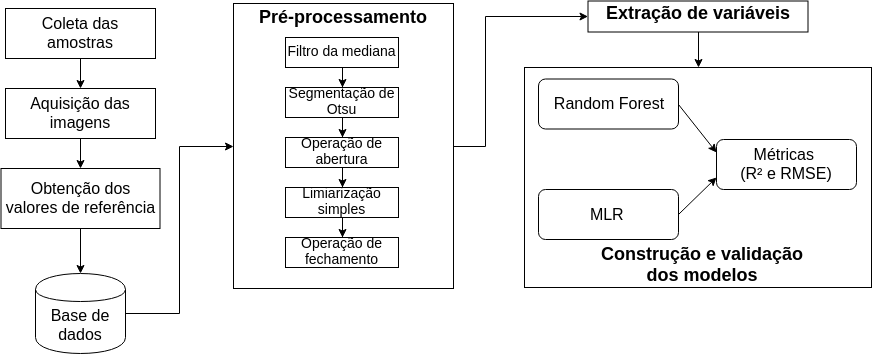
\includegraphics[scale=0.5]{img/diag.png}
    \legend{\textbf{Fonte:} (Autor, 2019).}
\end{figure}

\section{Descrição das amostras}

As mangas utilizadas no estudo eram da variedade ‘Palmer’, sendo uma das variedades mais produzidas no Vale do São Francisco (EMBRAPA SEMIÁRIDO, 2010), sendo caracterizada por frutos aromáticos e grandes, com peso de até 900 g, tom esverdeado ou arroxeado quando estão imaturos e cor vermelha quando maduros. 

As amostras foram coletadas de pomares comerciais da Fazenda SpecialFruit Importação e Exportação Ltda. em Petrolina e Juazeiro. Foram marcadas trinta plantas distribuídas em cinco fileiras de plantio de um lote do pomar. A cada quinze dias foram colhidos manualmente 60 frutos (dois de cada planta), para cada variedade, iniciando-se dos 35 dias após a floração\footnote{\label{ftnote:floracao} Etapa reprodutiva em que ocorre a diferenciação do meristema vegetativo para o floral, originando os componentes da flor (pétalas, estames e pistilo) (DUARTE FILHO et al., 1999).} até o ponto de colheita comercial adotado pela Fazenda, visando a construção de um modelo robusto de predição, onde mangas de diferentes estádios de maturação fossem utilizadas. As mangas foram colhidas num intervalo de 15 em 15 dias e, após a colheita, de 10 em 10 dias.

\section{Aquisição das imagens}

As imagens das mangas foram obtidas para cada lado da fruta no mesmo dia em que elas foram coletadas. Elas foram posicionadas em uma caixa de madeira compensada com um orifício no topo (Figura \ref{img:caixa}), onde foi posicionada uma câmera de 18 MP. O interior da caixa é preto fosco e contém uma superfície não reflexiva para o apoio das mangas. Na parte superior foram dispostos 3 LEDs brancos para a iluminação das amostras. O equipamento foi obtido a partir de uma parceria com o Laboratório de Energia na Agricultura (LENA) da UNIVASF. 

\begin{figure}[H]
\centering
	\caption{Câmara para aquisição das imagens.}\label{img:caixa}
	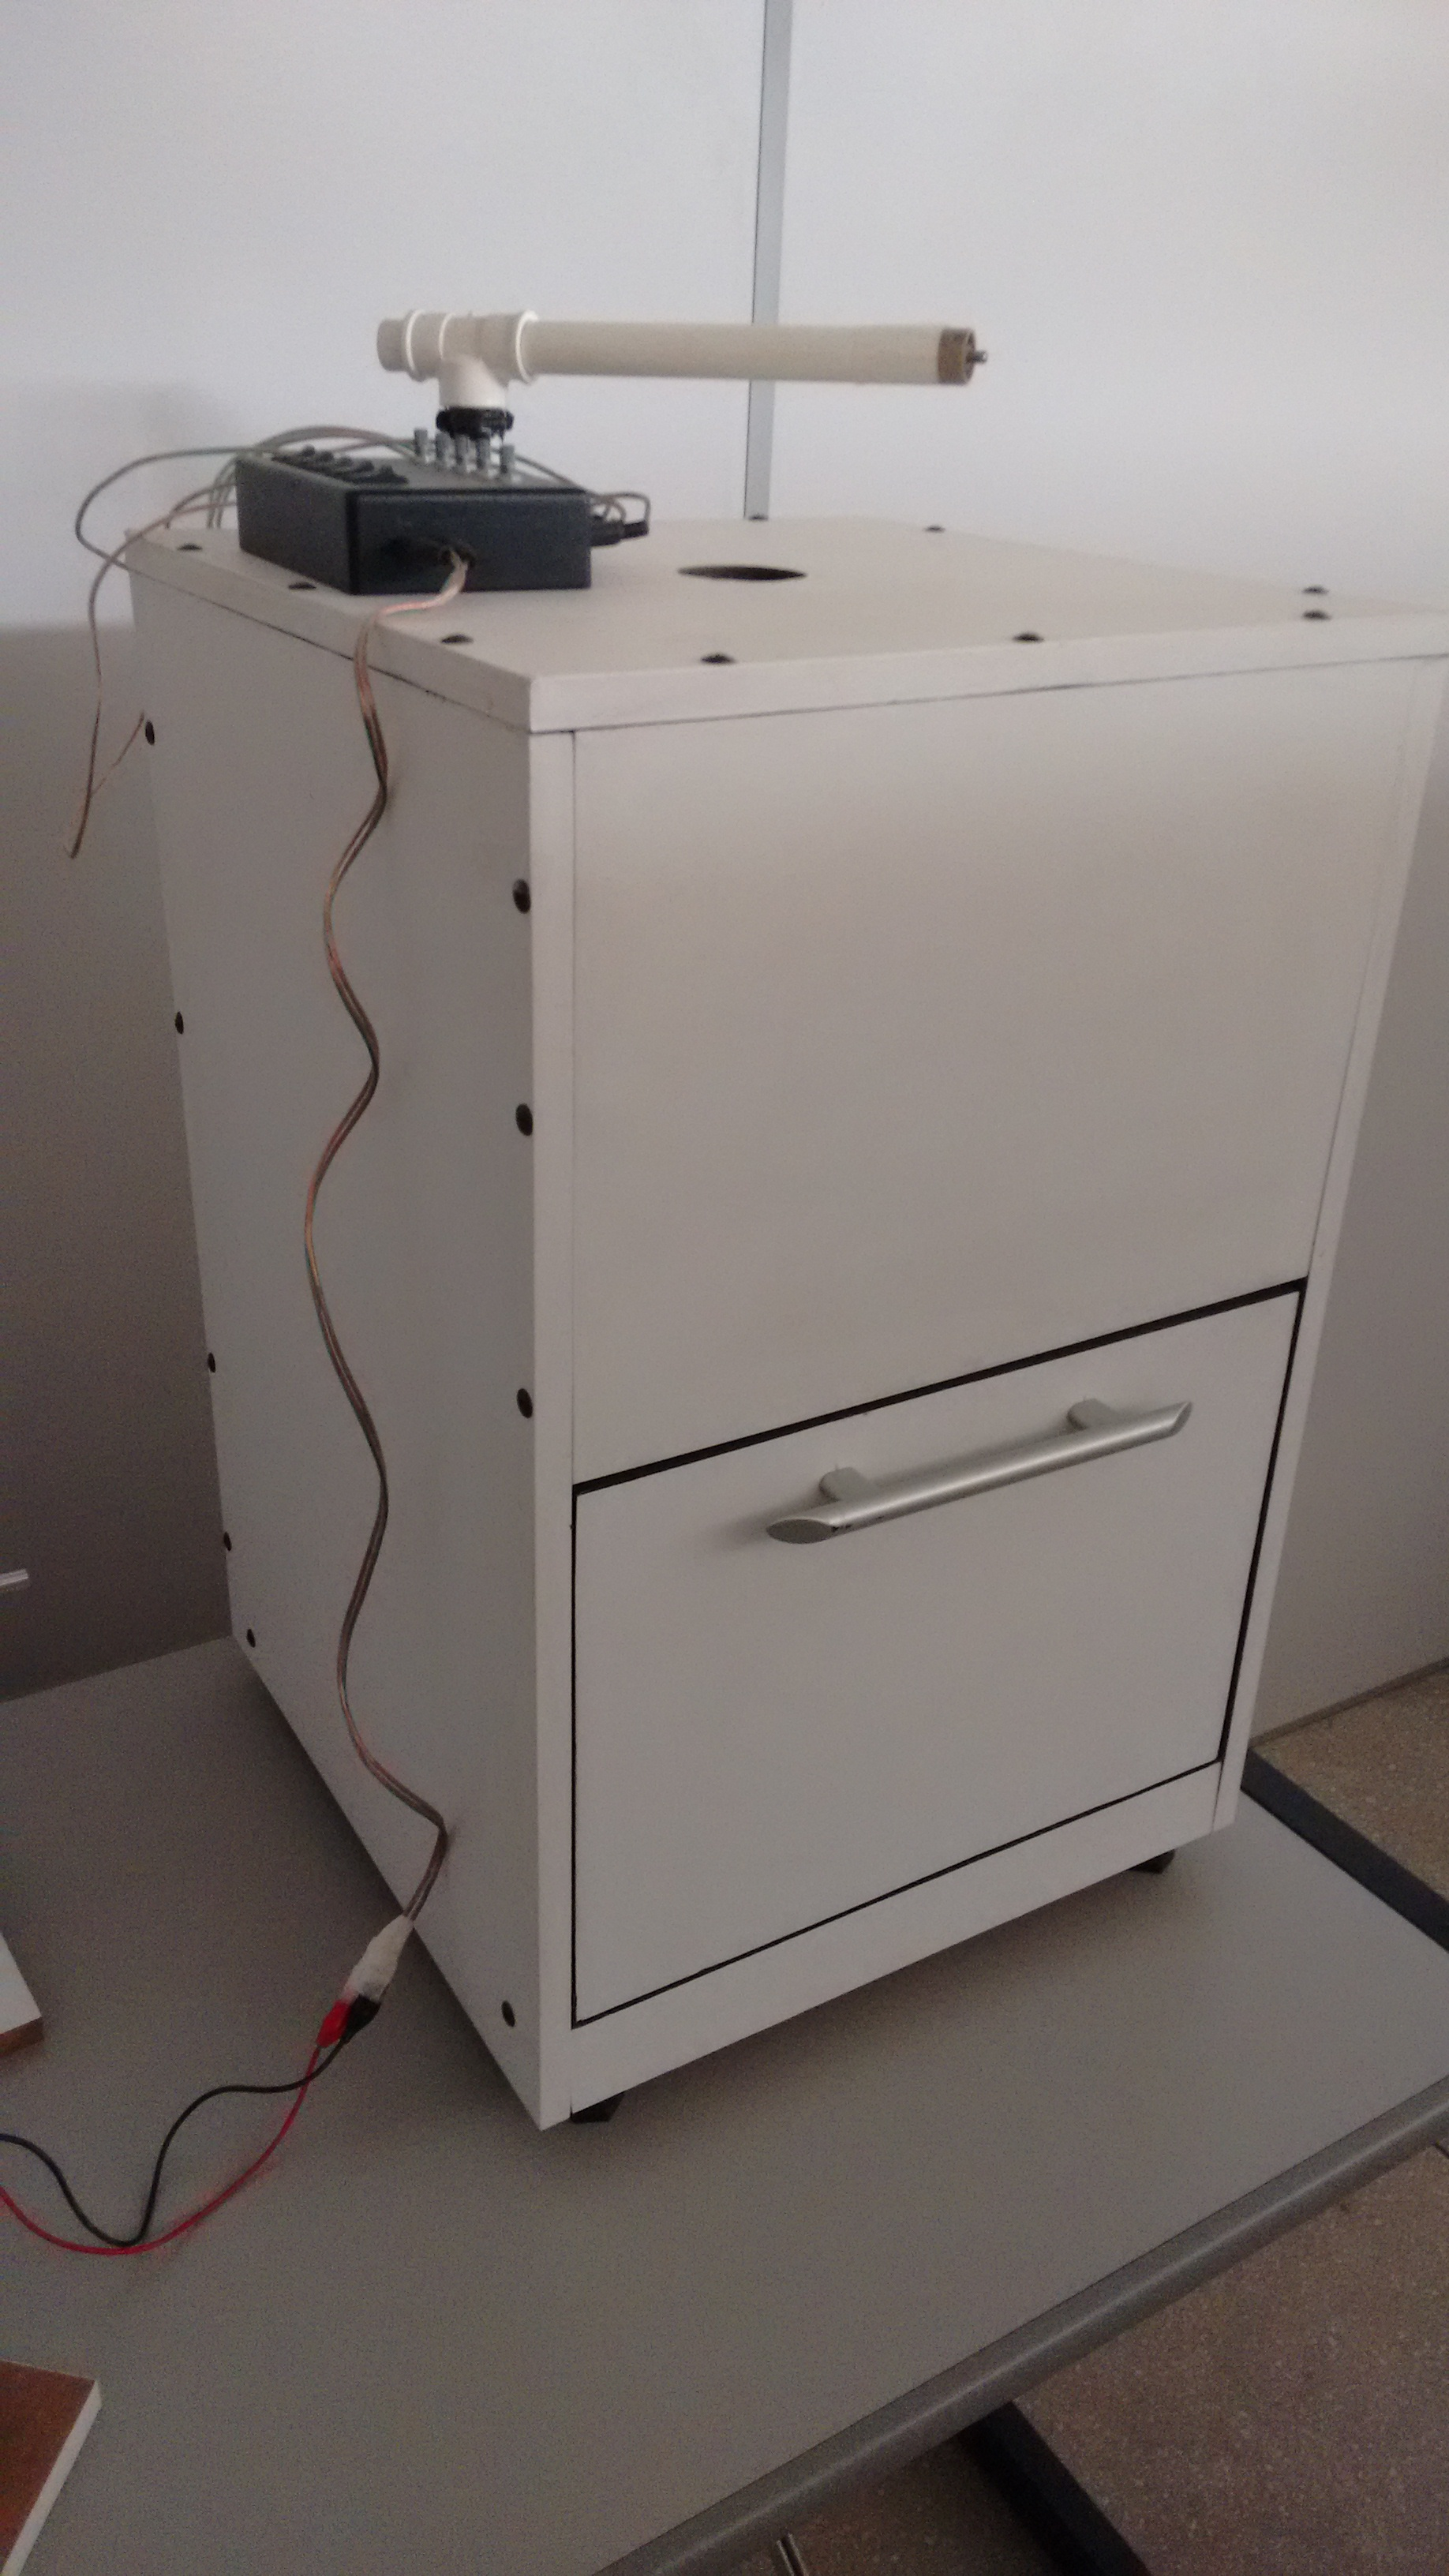
\includegraphics[scale=0.1]{img/caixa.jpg}
	\legend{\textbf{Fonte:} (Autor, 2019).}
\end{figure}

Foram tiradas fotos de 750 mangas, e, como os dois lados de cada amostra foram fotografados, no total obtiveram-se 1500 imagens. Para a 'Palmer', foram fotografadas 600 mangas até o dia da colheita e 150 após ela. A Figura \ref{img:palmer_tommy} exibe uma das fotos da 'Palmer'.

\begin{figure}[H]
\centering
    \caption{\label{img:palmer_tommy} Foto tirada da manga 'Palmer'.}
    {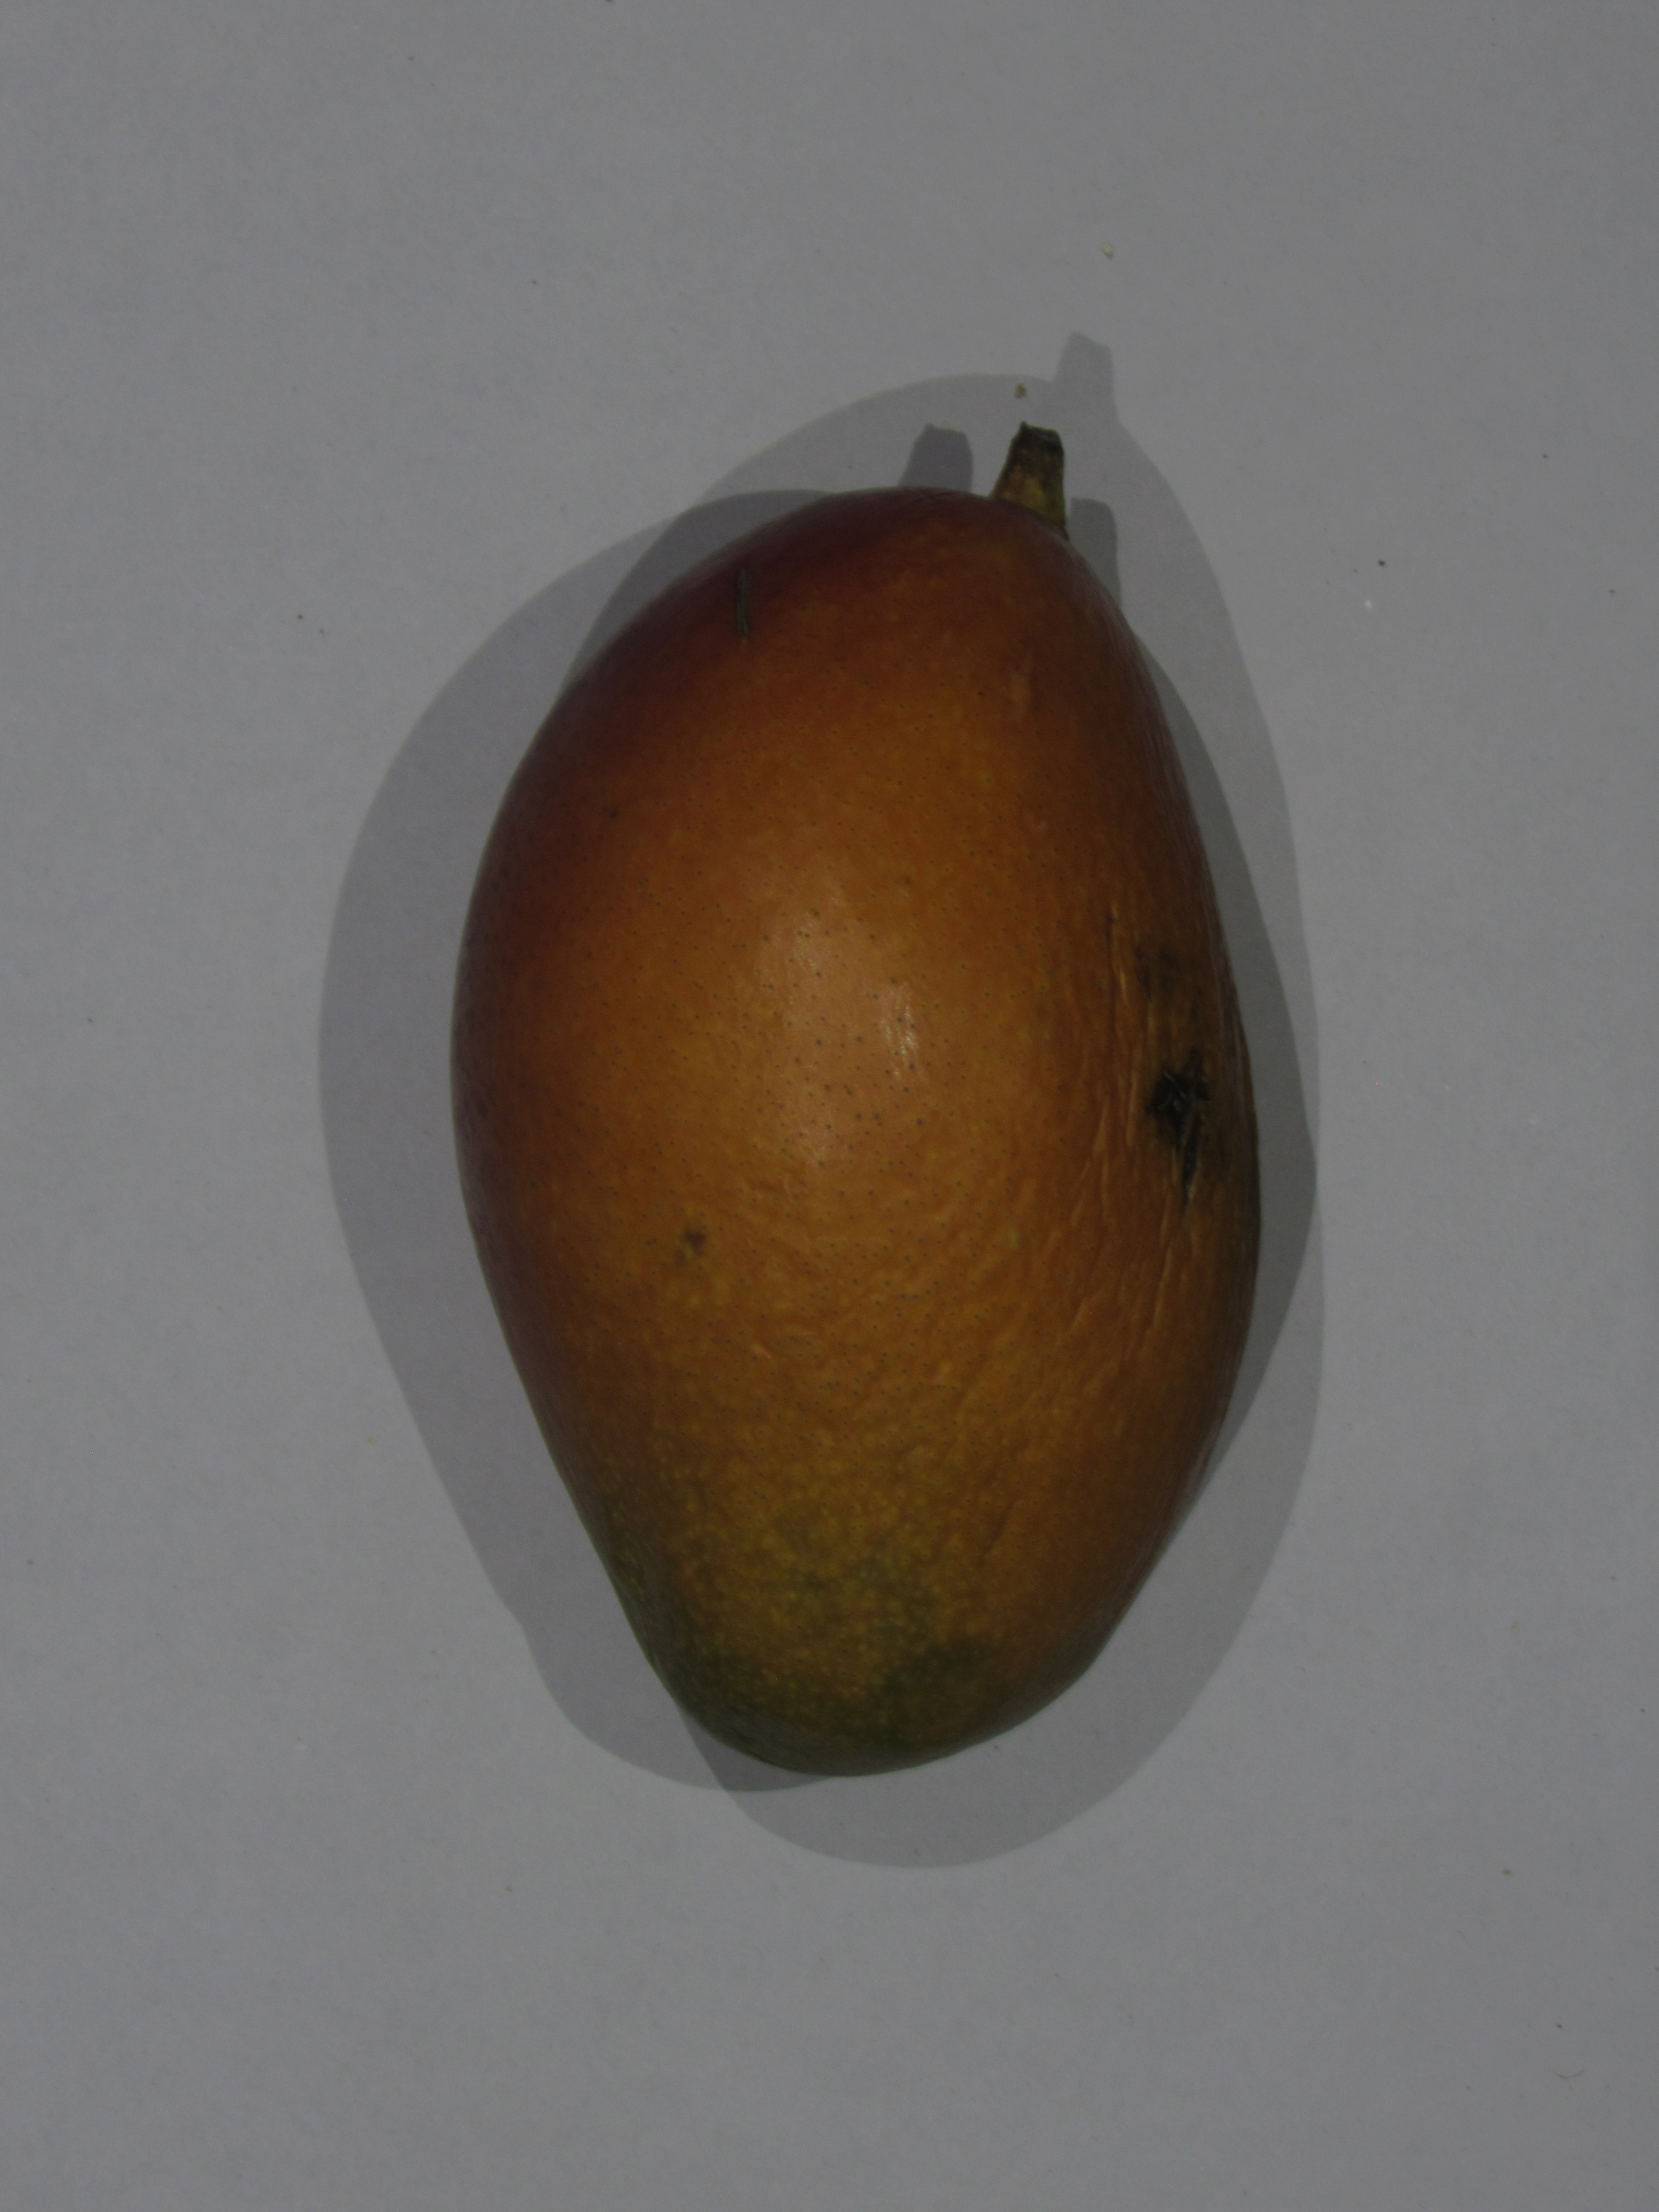
\includegraphics[scale=0.16]{img/palmer}}
    \legend{\textbf{Fonte: } (Autor, 2019).}
\end{figure}

\section{Obtenção dos valores de referência}

Os valores reais de SST foram obtidos segundo o procedimento do Instituto Adolfo Lutz (2008), sendo também adotado por Yahaya et al. (2015). Nele, as mangas têm inicialmente sua polpa homogeneizada e filtrada por uma centrífuga. O suco extraído é colocado em um refratômetro digital (HI 96804, Hanna Instruments, USA) para a quantificação de SST em ºBrix.

\section{Pré-processamento das imagens}

Como as imagens obtidas possuíam ruído e informações irrelevantes, foi necessário realizar o pré-processamento das mesmas. Foram testadas diferentes configurações de algoritmos, de forma a remover a maior quantidade possível de ruído sem perda de informações importantes da imagem. Apesar de as fotos terem sido tiradas em um ambiente controlado, as imagens resultantes variaram quanto ao ruído nelas contido, devido ao acúmulo de sujeira na câmara com o passar das semanas do experimento. Sendo assim, as configurações das técnicas variaram para cada imagem.

A primeira técnica aplicada foi o filtro da mediana, visando a remoção de manchas contidas nas imagens. O tamanho de janela que garantiu uma melhor remoção de ruído na maioria das imagens foi de 11x11 pixels. Após isso, as imagens foram segmentadas através do algoritmo de Otsu, de forma que as mangas fossem isoladas do fundo. Com isso, notou-se nas imagens a presença de pequenos pontos que não foram removidos pelo filtro da mediana. Apesar de a remoção dos mesmos ter sido possível com uma segunda filtragem pela mediana, notou-se uma perda de detalhes na manga. Sendo assim, optou-se por empregar a operação de abertura, através da qual pequenos pontos da imagem foram removidos, ao empregar um \textit{kernel} variando entre 15x15 e 105x105 pixels. 

A utilização destas técnicas não garantiu uma remoção completa das sombras contidas na imagem. Assim, utilizou-se a limiarização simples para este fim, visto que a intensidade dos pixels correspondentes às sombras era, em geral, visivelmente menor que a intensidade dos pixels das mangas. A configuração desta técnica que conferiu os melhores resultados possuiu um \textit{threshold} igual a 100, aplicado na imagem em escala de cinza. Como a limiarização simples resultou na remoção de partes da manga, além das sombras delas, empregou-se a operação morfológica de fechamento para o preenchimento das mangas. O melhor tamanho do \textit{kernel} obtido foi de 13x13 pixels.

Por fim, foram traçados os contornos das mangas, visando a remoção de partes da imagem que não continham a fruta. A Figura \ref{fig:prep} mostra uma imagem original e pré-processada.

\begin{figure}[!htb]
\centering
    \caption{\label{fig:prep} Antes e depois do pré-processamento (a) Imagem original (b) Imagem resultante após utilização de técnicas de pré-processamento.}
    \subcaptionbox{}{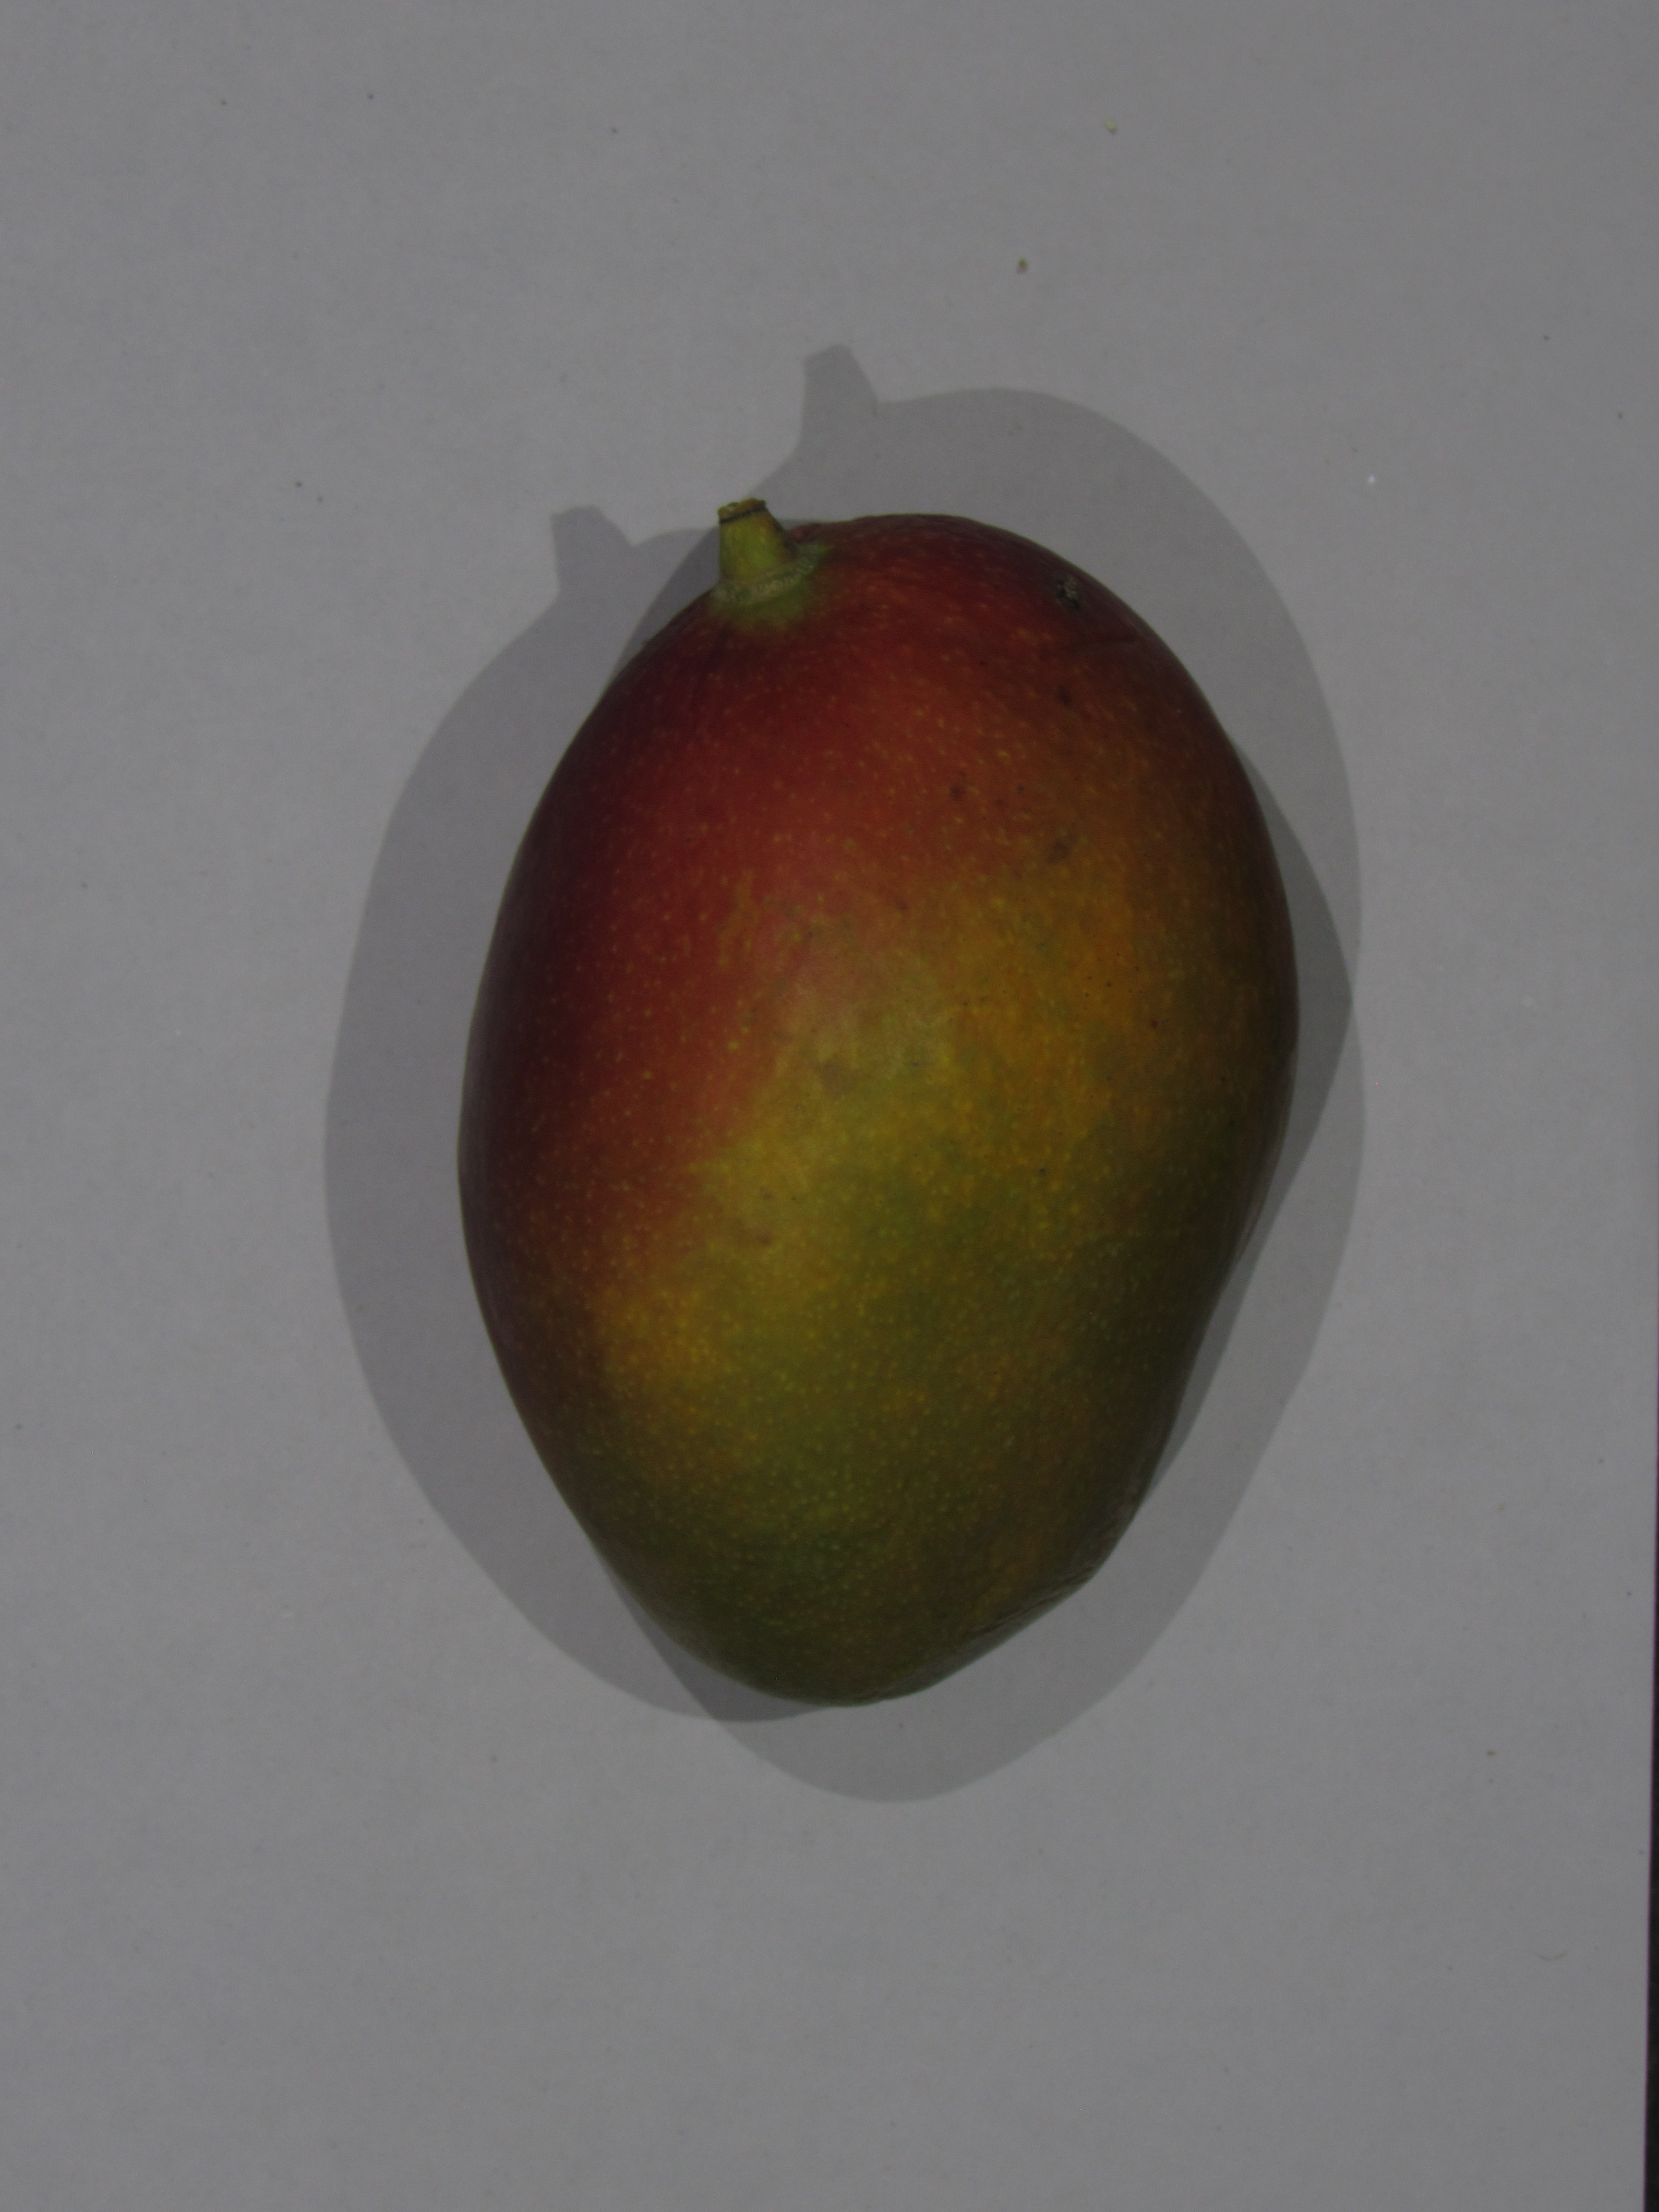
\includegraphics[scale=0.035]{img/sem_processamento.JPG}}
    \subcaptionbox{}{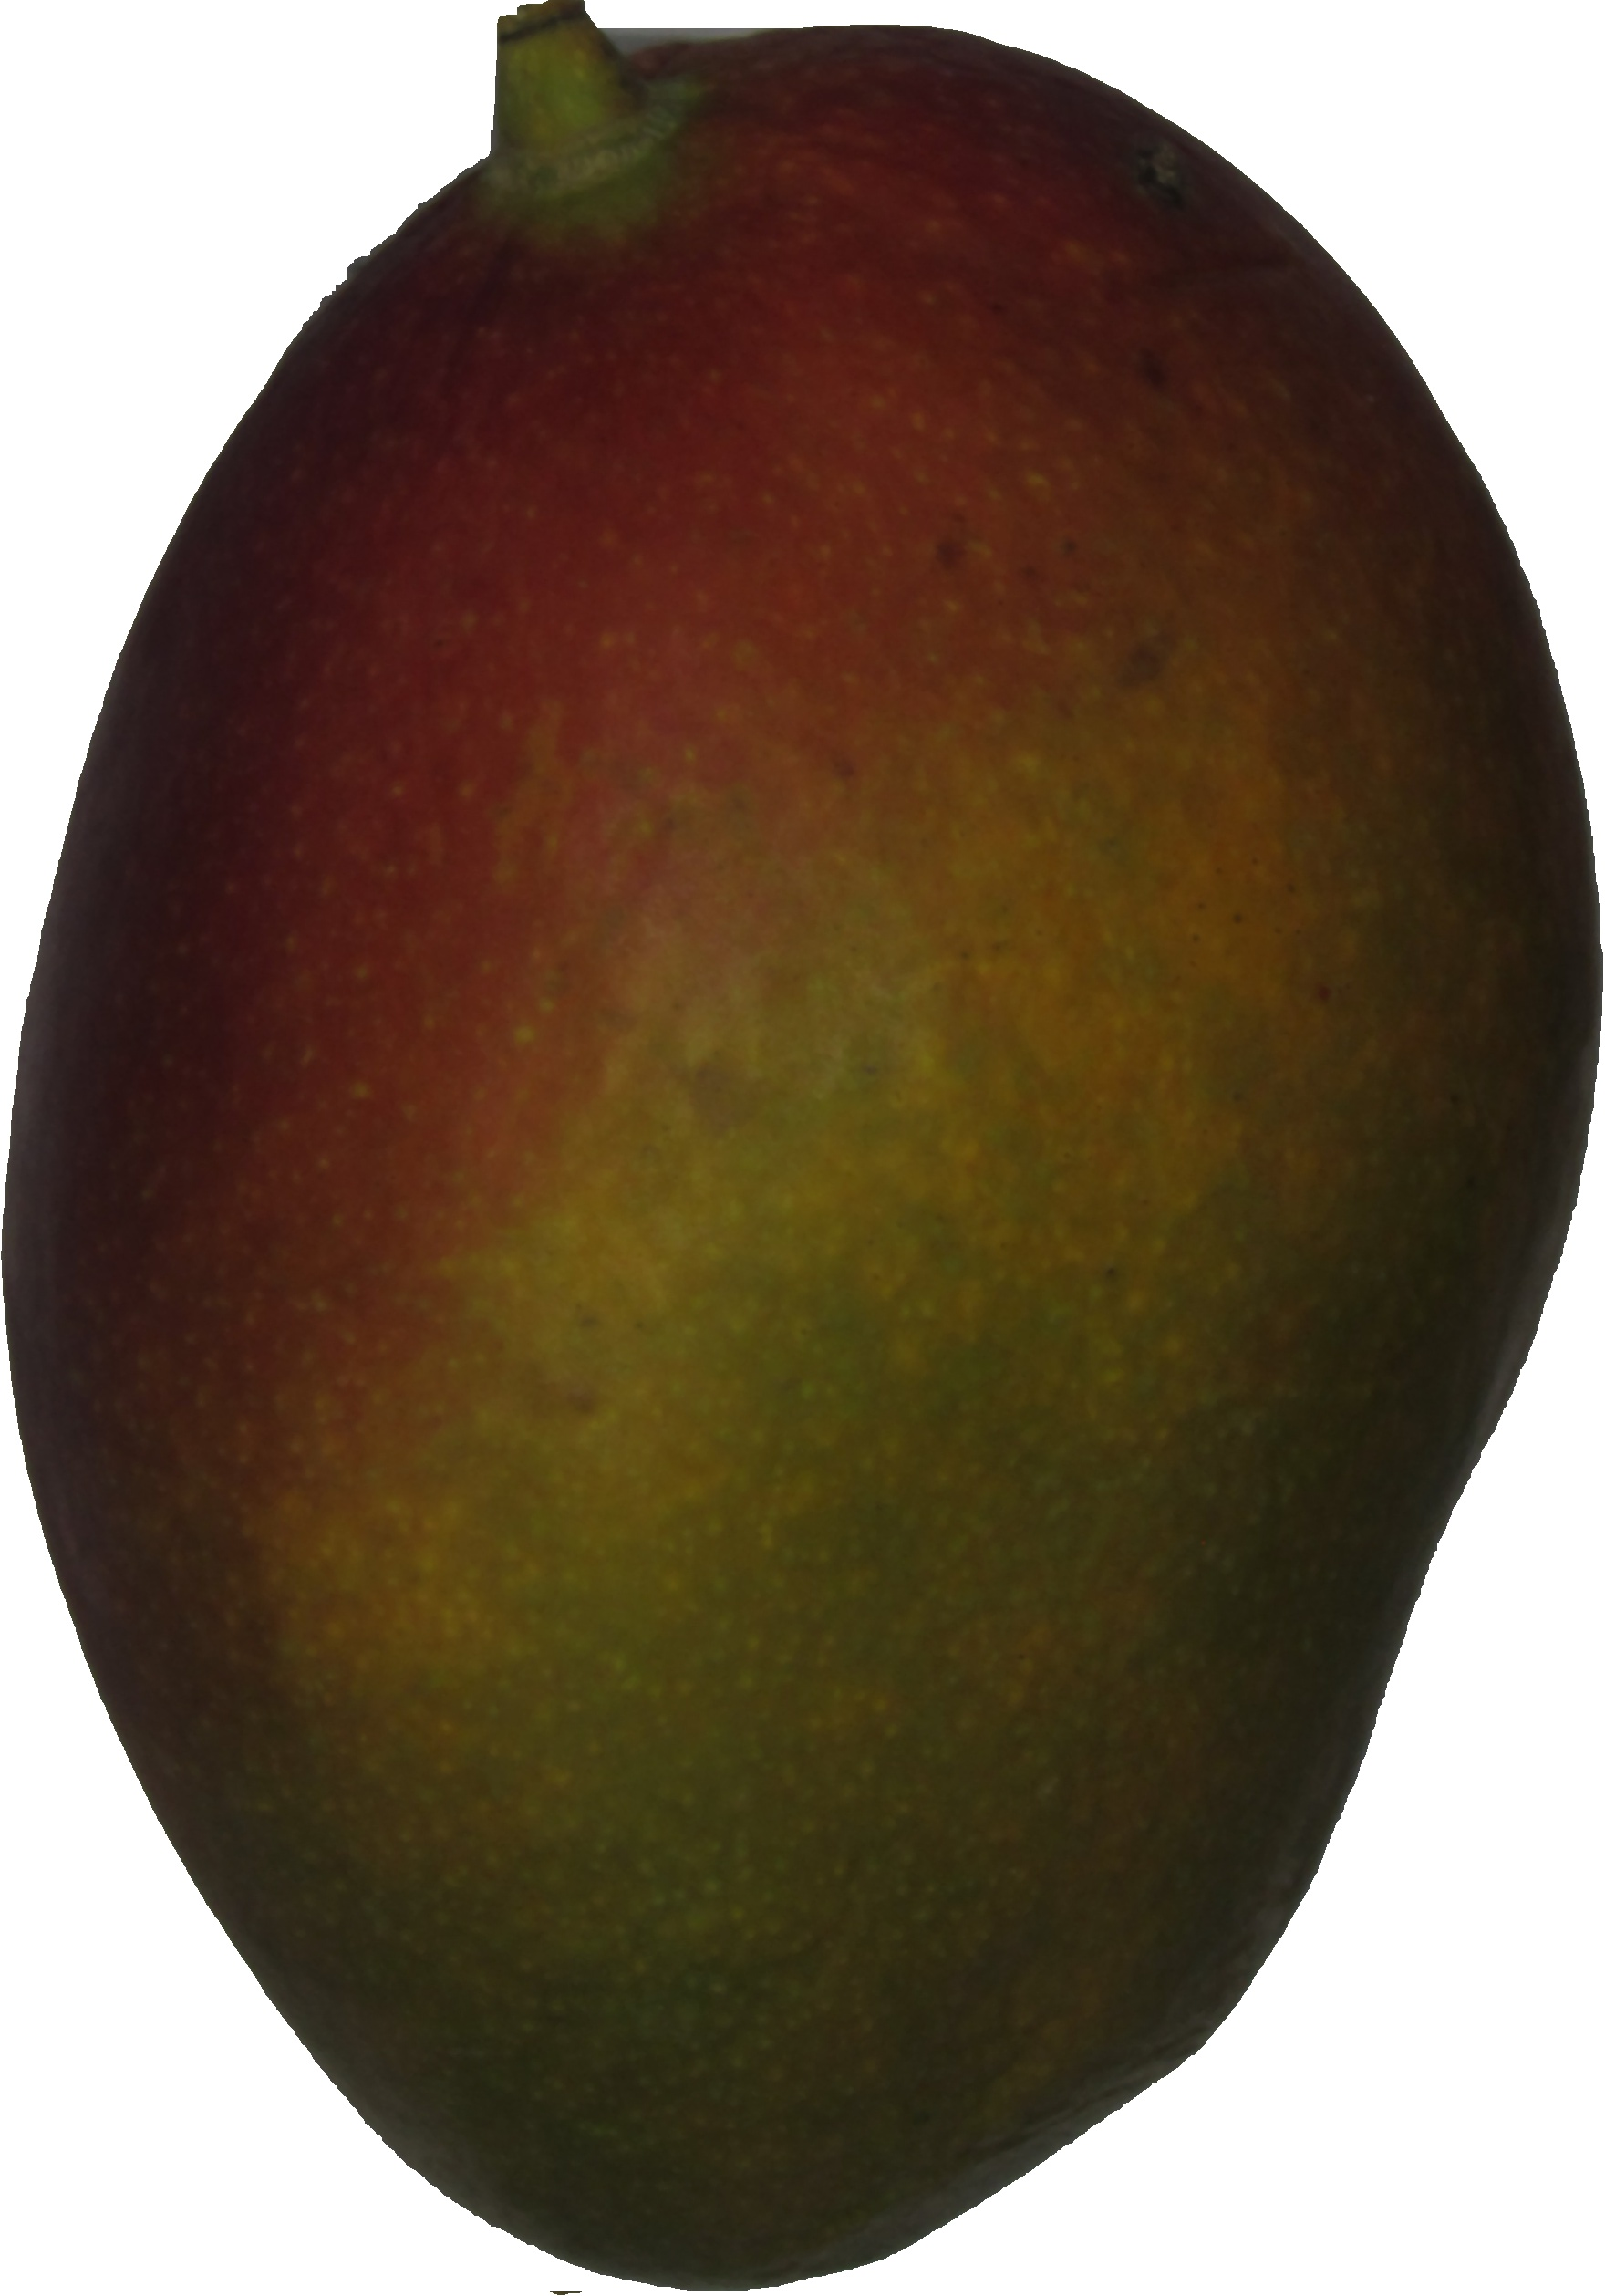
\includegraphics[scale=0.062]{img/processada.JPG}}
    \legend{\textbf{Fonte: } (Autor, 2019).}
\end{figure}

Posteriormente, as variáveis mencionadas na Tabela \ref{tab:artigos_att} foram extraídas para cada imagem. Todos os algoritmos de pré-processamento de imagens, assim como a extração de variáveis, foram realizados através da linguagem de programação Python, com o auxílio da biblioteca OpenCV.

\section{Construção dos modelos}

Antes da construção dos modelos foi realizada uma reamostragem das imagens, devido ao desbalanceamento presente na base de dados. Como havia 600 imagens de mangas tiradas antes da colheita e apenas 240 imagens tiradas após ela, foi feita uma repetição das imagens deste período até que fosse obtida uma quantidade igual de imagens nos dois períodos.

A construção dos modelos foi feita através da biblioteca \textit{Scikit-Learn}, assim como a validação e obtenção das métricas. Como foi utilizada a estratégia 5-\textit{fold cross-validation}, em cada uma das 5 iterações 240 amostras eram utilizadas para teste e as demais para treinamento do modelo. A partir dos valores reais e previstos, os valores de $R$ e $RMSE$ foram calculados.

Assim, foram construídos modelos de \textit{Random Forest} e Regressão linear para os subconjuntos de variáveis utilizados em artigos que determinavam SST. Além disso, foi construído um modelo que reúne todas as variáveis encontradas na literatura, de forma a encontrar os atributos mais significantes para predição e SST. Na Tabela \ref{tbl:var_gps} são mostradas as variáveis para cada artigo investigado.

\begin{longtable}{m{11cm} m{4cm}}
\hline
Variáveis                                                                                                                                    & Autores                             \\ \hline
Média das intensidades dos pixels nos espaços RGB, HSV, L*a*b*                                                                               & Abarra et al. (2018)                \\ \hline
Cor HSV dominante                                                                                                                            & Yossy (2017)                        \\ \hline
Média das intensidades RGB na manga inteira, nas regiões apex, equatorial e cume, diferença das médias e gradiente longitudinal     & Nandi, Tudu e Koley (2014)          \\ \hline
Número de pixels correspondente à manga                                                                                                      & Teoh e Syaifudin (2007)             \\ \hline
Média das intensidades dos pixels no espaço RGB                                                                                              & Yahaya et al. (2015)                \\ \hline
Média das intensidades dos pixels no espaço L*a*b* e variáveis fractais 																 	& Zheng e Lu (2012)                   \\ \hline
Média das intensidades dos pixels no espaço HSV                                                                                              & Khairunniza-Bejo e Kamarudin (2011) \\ \hline
Média das intensidades dos pixels nos espaços HSV e L*a*b*                                                                                   & Vélez-Rivera et al. (2014)          \\ \hline
Média das intensidades dos pixels nos espaços RGB e HSV e taxas R/G, R/B e S/H                                                              & Salunkhe e Patil (2015)             \\ \hline
Média das intensidades dos pixels no canal b*, número de pixels e diâmetro                                                                   & Pandey, Gamit e Naik (2014) \\ \hline       
\caption{Subconjuntos de variáveis obtidos a partir da literatura.}\label{tbl:var_gps}
\end{longtable} 

% \subsection{Subseção de exemplo 1 - Referenciando seções} \label{subsec:subsec1}


%--------------------------------------------------------------------------------------
% Insere a seção de cronograma
% Está comentada porque só é necessária no TCC I
%--------------------------------------------------------------------------------------

%\section{Cronograma} \label{sec:crono}

%A tabela \ref{tab:cronograma} mostra o cronograma de atividades a serem executadas para o TCC II, com base no calendário de 201X.Y da UNIVASF.

%\newpage
%\begin{table}[!thb]
%	%\huge
%    \centering
%    \caption{\label{tab:cronograma} Cronograma das atividades previstas para o TCC II}
%%    \begin{adjustbox}{max width=\textwidth}
%    \begin{tabular}{p{6.5cm}|c|c|c|c|c|c}
%    \toprule
%    \textbf{Atividade}                      & Nov & Dez & Jan & Fev & Mar & Abr \\ \hline
%    Implementar o banco de dados              & X    & X     &       &        &          &          \\ \hline
%    Desenvolver a API HTTP RESTful                      &   X   & X     &       &        &          &          \\ \hline
%    Implementar o serviço de captura de dados        &      &      & X     &   X     &          &          \\ \hline
%    Desenvolver a aplicação \textit{Web/mobile} para exibição dos dados         &      &      & X     &   X     &     X     &          \\ \hline
 %   Teste do sistema            &      &       &       &        & X        &          %\\ \hline
 %   Escrita do TCC II                       &   X   & X     & X     & X      & X        & X        \\ \hline
%   Defesa do TCC II                        &      &       &       &        &          & X       \\
%    \bottomrule
 %   \end{tabular}
 %   \end{adjustbox}
%    \legend{\textbf{Fonte:} O autor.}
%\end{table}

